% Method figure: (a) an episode re-sends its context, (b) the turn--component graph, (c) the two splits of a skill's change.
% Hand-written TikZ; every block, edge width and bar value is illustrative (no data).
% Colors follow the teaser figure: skill text vermilion, bash output green, read output blue, rest of the prompt gray;
% four terms: more actions blue, turn-splitting orange, content per turn pink, skill text vermilion, measured total black.
% Size: 6.3 in wide (the text width), smallest font 7 pt (math scripts declared at 7 pt).
% Build: python -m aux.tokens.method  ->  mech_method.pdf
\RequirePackage{fix-cm}
\documentclass[tikz,border=2pt]{standalone}
\usepackage{times}
\usepackage[T1]{fontenc}
\usepackage[utf8]{inputenc}
\usepackage{amsmath,amssymb}
\usetikzlibrary{arrows.meta,decorations.pathreplacing,calc}
% math scripts never fall below 7 pt
\DeclareMathSizes{7.5}{7.5}{7}{7}
\DeclareMathSizes{8}{8}{7}{7}
\DeclareMathSizes{8.5}{8.5}{7}{7}
% components
\definecolor{cSkill}{HTML}{D55E00}
\definecolor{cBash}{HTML}{009E73}
\definecolor{cRead}{HTML}{0072B2}
\definecolor{cOther}{HTML}{BBBBBB}
% four terms
\definecolor{cAct}{HTML}{0072B2}
\definecolor{cSplit}{HTML}{E69F00}
\definecolor{cCont}{HTML}{CC79A7}
\definecolor{cText}{HTML}{D55E00}
\definecolor{cTot}{HTML}{222222}
% frames and text
\definecolor{cFrame}{HTML}{AAB0B8}
\definecolor{cBg}{HTML}{F7F8FA}
\definecolor{cGR}{HTML}{555555}
\definecolor{cDark}{HTML}{222222}

% panel geometry (cm): total inner width 15.861 = 6.3 in - 2 x 2 pt border
\def\H{5.85}
\def\Wa{4.55}\def\Wb{4.96}\def\Wc{5.95}
\def\Xb{4.75}\def\Xc{9.91}

% panel (a): column width, pitch, first column, base line, prefix parts, content per turn
\def\cw{0.38}\def\cp{0.49}\def\xa{0.66}\def\yb{0.72}
\def\Fo{0.54}\def\Fs{0.32}\def\FF{0.86}\def\hh{0.44}

% history block k (the content turn k adds): x = left edge, opacity
% turn 1 bash, turn 2 read, turn 3 bash + read, turn 4 bash, turn 5 bash
\newcommand{\hist}[3]{%
  \pgfmathsetmacro{\yy}{\yb+\FF+(#2-1)*\hh}%
  \ifcase#2\or
    \fill[cBash,fill opacity=#3] (#1,\yy) rectangle ++(\cw,\hh);\or
    \fill[cRead,fill opacity=#3] (#1,\yy) rectangle ++(\cw,\hh);\or
    \fill[cBash,fill opacity=#3] (#1,\yy) rectangle ++(\cw,0.5*\hh);
    \fill[cRead,fill opacity=#3] (#1,\yy+0.5*\hh) rectangle ++(\cw,0.5*\hh);\or
    \fill[cBash,fill opacity=#3] (#1,\yy) rectangle ++(\cw,\hh);\or
    \fill[cBash,fill opacity=#3] (#1,\yy) rectangle ++(\cw,\hh);\fi}

\begin{document}
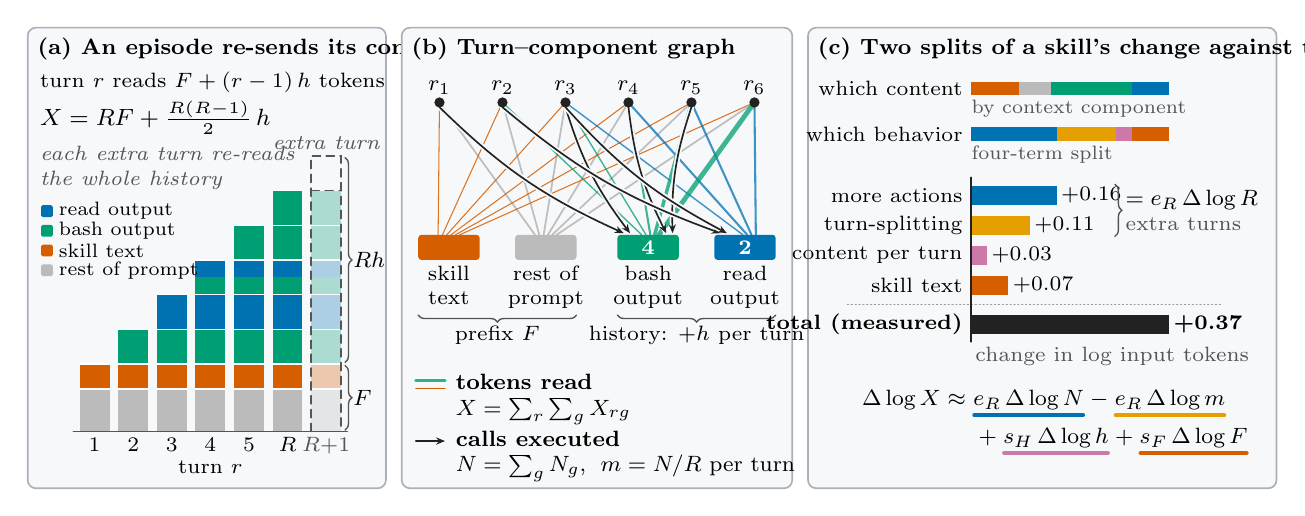
\begin{tikzpicture}[x=1cm,y=1cm,line cap=round,>={Stealth[length=3.2pt,width=2.6pt]},
  panel/.style={draw=cFrame,fill=cBg,line width=0.6pt,rounded corners=3pt},
  ttl/.style={font=\fontsize{8}{9.5}\selectfont\bfseries,anchor=north west,inner sep=0pt},
  lab/.style={font=\fontsize{7.5}{8.8}\selectfont,inner sep=0pt},
  mth/.style={font=\fontsize{8}{9.5}\selectfont,inner sep=0pt},
  note/.style={font=\fontsize{7.5}{8.8}\selectfont\itshape,text=cGR,inner sep=0pt},
  brc/.style={decorate,decoration={brace,amplitude=2.5pt},line width=0.5pt,draw=cGR},
  sep/.style={draw=white,line width=0.5pt},
  call/.style={->,draw=cDark,line width=0.6pt,preaction={draw=cBg,line width=1.9pt,-}},
  ]

%% ================================================================ PANEL (a)
\begin{scope}
\draw[panel] (0,0) rectangle (\Wa,\H);
\node[ttl] at (0.12,\H-0.12) {(a) An episode re-sends its context};

% columns r = 1..6: prefix (rest of prompt, skill text) + the history so far
\foreach \r in {1,...,6} {
  \pgfmathsetmacro{\x}{\xa+(\r-1)*\cp}
  \fill[cOther] (\x,\yb) rectangle ++(\cw,\Fo);
  \fill[cSkill] (\x,\yb+\Fo) rectangle ++(\cw,\Fs);
  \ifnum\r>1
    \pgfmathtruncatemacro{\last}{\r-1}
    \foreach \k in {1,...,\last} { \hist{\x}{\k}{1} }
  \fi
  % white seams between blocks
  \pgfmathtruncatemacro{\nb}{\r-1}
  \draw[sep] (\x,\yb+\Fo) -- ++(\cw,0);
  \foreach \k in {0,...,\nb} \draw[sep] (\x,\yb+\FF+\k*\hh) -- ++(\cw,0);
}
% one extra turn: re-reads the prefix and the whole history (turn R's content included)
\pgfmathsetmacro{\xg}{\xa+6*\cp}
\fill[cOther,fill opacity=0.3] (\xg,\yb) rectangle ++(\cw,\Fo);
\fill[cSkill,fill opacity=0.3] (\xg,\yb+\Fo) rectangle ++(\cw,\Fs);
\foreach \k in {1,...,5} { \hist{\xg}{\k}{0.3} }
\draw[sep] (\xg,\yb+\Fo) -- ++(\cw,0);
\foreach \k in {0,...,5} \draw[sep] (\xg,\yb+\FF+\k*\hh) -- ++(\cw,0);
\draw[cGR,densely dashed,line width=0.5pt] (\xg,\yb) rectangle ++(\cw,\FF+6*\hh);
\draw[cGR,densely dashed,line width=0.4pt] (\xg,\yb+\FF+5*\hh) -- ++(\cw,0);
\node[note,anchor=south] at (\xg+0.5*\cw,\yb+\FF+6*\hh+0.07) {extra turn};
% braces on the extra turn: prefix F and history R h
\draw[brc] (\xg+\cw+0.05,\yb+\FF-0.02) -- (\xg+\cw+0.05,\yb+0.02);
\node[mth,anchor=west] at (\xg+\cw+0.15,\yb+0.5*\FF) {$F$};
\draw[brc] (\xg+\cw+0.05,\yb+\FF+6*\hh-0.02) -- (\xg+\cw+0.05,\yb+\FF+0.02);
\node[mth,anchor=west] at (\xg+\cw+0.15,\yb+\FF+3*\hh) {$Rh$};

% axis
\draw[cGR,line width=0.5pt] (\xa-0.08,\yb) -- (\xg+\cw+0.08,\yb);
\foreach \r/\t in {1/1,2/2,3/3,4/4,5/5,6/$R$} \node[lab,anchor=north] at ({\xa+(\r-1)*\cp+0.5*\cw},\yb-0.07) {\t};
\node[lab,anchor=north,text=cGR] at (\xg+0.5*\cw,\yb-0.07) {$R{+}1$};
\node[lab,anchor=north] at (0.5*\xa+0.5*\xg+0.5*\cw,\yb-0.36) {turn $r$};

% the sum over turns
\node[lab,anchor=north west] at (0.15,\H-0.55) {turn $r$ reads $F+(r-1)\,h$ tokens};
\node[font=\fontsize{8.5}{10}\selectfont,inner sep=0pt,anchor=north west] at (0.15,\H-0.93) {$X=RF+\tfrac{R(R-1)}{2}\,h$};
\node[note,anchor=north west,align=left] at (0.15,\H-1.5) {each extra turn re-reads\\the whole history};
% color key, top to bottom in the order of the stack
\foreach \y/\col/\t in {3.52/cRead/read output, 3.27/cBash/bash output, 3.02/cSkill/skill text, 2.77/cOther/rest of prompt} {
  \fill[\col,rounded corners=0.6pt] (0.17,\y-0.075) rectangle ++(0.15,0.15);
  \node[lab,anchor=west,font=\fontsize{7}{8}\selectfont] at (0.39,\y) {\t};
}
\end{scope}

%% ================================================================ PANEL (b)
\begin{scope}[shift={(\Xb,0)}]
\draw[panel] (0,0) rectangle (\Wb,\H);
\node[ttl] at (0.12,\H-0.12) {(b) Turn--component graph};

\def\yd{4.9}      % turn nodes
\def\ybt{3.22}    % top of the component nodes
\def\ybb{2.9}     % bottom of the component nodes
% component centers: skill text, rest of prompt, bash output, read output
\def\cS{0.6}\def\cO{1.83}\def\cB{3.13}\def\cR{4.36}
\def\bw{0.78}

% context edges: width ~ tokens X_rg (0.5 pt per h); prefix read by every turn, outputs by every later turn
\foreach \r in {1,...,6} {
  \pgfmathsetmacro{\x}{0.48+(\r-1)*0.8}
  \pgfmathsetmacro{\o}{(\r-3.5)*0.055}
  \draw[cSkill,line width=0.38pt,opacity=0.85] (\x,\yd) -- (\cS+\o,\ybt);
  \draw[cOther,line width=0.63pt,opacity=0.95] (\x,\yd) -- (\cO+\o,\ybt);
}
\foreach \r/\wb/\wr in {2/0.5/0, 3/0.5/0.5, 4/0.75/0.75, 5/1.25/0.75, 6/1.75/0.75} {
  \pgfmathsetmacro{\x}{0.48+(\r-1)*0.8}
  \pgfmathsetmacro{\o}{(\r-3.5)*0.055}
  \draw[cBash,line width=\wb pt,opacity=0.75] (\x,\yd) -- (\cB+\o,\ybt);
  \ifdim\wr pt>0pt \draw[cRead,line width=\wr pt,opacity=0.75] (\x,\yd) -- (\cR+\o,\ybt); \fi
}
% call edges: turn 1 bash, 2 read, 3 bash + read, 4 bash, 5 bash, 6 answers
\foreach \r/\tx in {1/2.82, 3/2.9, 4/3.36, 5/3.44} {
  \pgfmathsetmacro{\x}{0.48+(\r-1)*0.8}
  \draw[call] (\x,\yd-0.06) to[bend right=10] (\tx,\ybt+0.02);
}
\foreach \r/\tx in {2/4.05, 3/4.13} {
  \pgfmathsetmacro{\x}{0.48+(\r-1)*0.8}
  \draw[call] (\x,\yd-0.06) to[bend right=10] (\tx,\ybt+0.02);
}
% turn nodes
\foreach \r in {1,...,6} {
  \pgfmathsetmacro{\x}{0.48+(\r-1)*0.8}
  \fill[cDark] (\x,\yd) circle (0.065);
  \node[mth,anchor=south] at (\x,\yd+0.1) {$r_{\r}$};
}
% component nodes (tool nodes carry their call counts N_g)
\foreach \c/\col in {\cS/cSkill,\cO/cOther,\cB/cBash,\cR/cRead}
  \fill[\col,rounded corners=1.2pt] (\c-0.5*\bw,\ybb) rectangle (\c+0.5*\bw,\ybt);
\node[lab,text=white,font=\fontsize{7.5}{8.8}\selectfont\bfseries] at (\cB,0.5*\ybb+0.5*\ybt) {4};
\node[lab,text=white,font=\fontsize{7.5}{8.8}\selectfont\bfseries] at (\cR,0.5*\ybb+0.5*\ybt) {2};
\foreach \c/\t in {\cS/{skill\\text},\cO/{rest of\\prompt},\cB/{bash\\output},\cR/{read\\output}}
  \node[lab,anchor=north,align=center] at (\c,\ybb-0.07) {\t};
% F and h
\draw[brc] (\cO+0.5*\bw,2.2) -- (\cS-0.5*\bw,2.2);
\node[lab,anchor=north] at (0.5*\cS+0.5*\cO,2.07) {prefix $F$};
\draw[brc] (\cR+0.5*\bw,2.2) -- (\cB-0.5*\bw,2.2);
\node[lab,anchor=north] at (0.5*\cB+0.5*\cR,2.07) {history: $+h$ per turn};

% the two streams
\draw[cBash,line width=1.2pt,opacity=0.8] (0.18,1.37) -- (0.55,1.37);
\draw[cSkill,line width=0.5pt] (0.18,1.27) -- (0.55,1.27);
\node[mth,anchor=base west] at (0.68,1.25) {\textbf{tokens read}};
\node[mth,anchor=base west] at (0.68,0.93) {$X=\sum_{r}\sum_{g}X_{rg}$};
\draw[call] (0.18,0.6) -- (0.55,0.6);
\node[mth,anchor=base west] at (0.68,0.53) {\textbf{calls executed}};
\node[mth,anchor=base west] at (0.68,0.21) {$N=\sum_{g}N_g$,\; $m=N/R$ per turn};
\end{scope}

%% ================================================================ PANEL (c)
\begin{scope}[shift={(\Xc,0)}]
\draw[panel] (0,0) rectangle (\Wc,\H);
\node[ttl] at (0.12,\H-0.12) {(c) Two splits of a skill's change against the seed};

\def\xl{1.97}  % right edge of the row labels
\def\xz{2.07}  % zero
\def\u{6.8}    % cm per log unit

% which content (component split, exact) vs which behavior (four-term split)
\node[lab,anchor=east] at (\xl,5.08) {which content};
\node[lab,anchor=north west,font=\fontsize{7}{8}\selectfont,text=cGR] at (\xz,4.94) {by context component};
\node[lab,anchor=east] at (\xl,4.5) {which behavior};
\node[lab,anchor=north west,font=\fontsize{7}{8}\selectfont,text=cGR] at (\xz,4.36) {four-term split};
\def\bh{0.17}
% segments as start/length/color, both summing to the measured total 0.37
\foreach \s/\v/\col in {0/0.09/cSkill, 0.09/0.06/cOther, 0.15/0.15/cBash, 0.30/0.07/cRead}
  \fill[\col] (\xz+\u*\s,5.08-0.5*\bh) rectangle ++(\u*\v,\bh);
\foreach \s/\v/\col in {0/0.16/cAct, 0.16/0.11/cSplit, 0.27/0.03/cCont, 0.30/0.07/cText}
  \fill[\col] (\xz+\u*\s,4.5-0.5*\bh) rectangle ++(\u*\v,\bh);

% four-term split: bars
\def\rh{0.24}
\foreach \y/\n/\v/\col in {3.72/more actions/0.16/cAct, 3.34/turn-splitting/0.11/cSplit, 2.96/content per turn/0.03/cCont, 2.58/skill text/0.07/cText} {
  \node[lab,anchor=east] at (\xl,\y) {\n};
  \fill[\col] (\xz,\y-0.5*\rh) rectangle ++(\u*\v,\rh);
  \node[lab,anchor=west] at (\xz+\u*\v+0.05,\y) {+\v};
}
\draw[cGR!60,line width=0.4pt,densely dotted] (0.5,2.33) -- (\xz+\u*0.37+0.66,2.33);
\node[lab,anchor=east,font=\fontsize{7.5}{8.8}\selectfont\bfseries] at (\xl,2.08) {total (measured)};
\fill[cTot] (\xz,2.08-0.5*\rh) rectangle ++(\u*0.37,\rh);
\node[lab,anchor=west,font=\fontsize{7.5}{8.8}\selectfont\bfseries] at (\xz+\u*0.37+0.05,2.08) {+0.37};
\draw[cDark,line width=0.5pt] (\xz,3.95) -- (\xz,1.86);
\node[lab,anchor=north west,text=cGR] at (\xz+0.05,1.8) {change in log input tokens};
% more actions + turn-splitting = e_R dlog R
\draw[brc] (\xz+\u*0.16+0.74,3.86) -- (\xz+\u*0.16+0.74,3.2);
\node[mth,anchor=west,align=left] at (\xz+\u*0.16+0.87,3.53) {$=e_R\,\Delta\log R$\\[-0.5pt]{\fontsize{7.5}{8.8}\selectfont\color{cGR}extra turns}};

% the four-term formula, each term marked in its color
\begin{scope}[every node/.style={mth,anchor=base west}]
\node (f0) at (0.68,1.05) {$\Delta\log X\approx{}$};
\node (f1) at (f0.base east) {$e_R\,\Delta\log N$};
\node (f2) at (f1.base east) {${}-{}$};
\node (f3) at (f2.base east) {$e_R\,\Delta\log m$};
\node (f4) at ($(f1.base west)+(0,-0.48)$) {${}+{}$};
\node (f5) at (f4.base east) {$s_H\,\Delta\log h$};
\node (f6) at (f5.base east) {${}+{}$};
\node (f7) at (f6.base east) {$s_F\,\Delta\log F$};
\end{scope}
\foreach \n/\col in {f1/cAct,f3/cSplit,f5/cCont,f7/cText}
  \draw[\col,line width=1.6pt] ($(\n.south west)+(0.02,-0.06)$) -- ($(\n.south east)+(-0.02,-0.06)$);
\end{scope}

% exact bounding box: 6.3 in minus the 2 pt border on each side
\pgfresetboundingbox
\path (0,0) rectangle ({6.3in-4pt},{\H cm});
\end{tikzpicture}
\end{document}
